\documentclass{beamer}
\usepackage[utf8]{inputenc}
\usepackage{amsmath, amssymb, bm}
\usepackage{physics}
\usepackage{graphicx}
\usepackage{hyperref}
\usepackage{xmpmulti}
\usepackage{tikz}
\usepackage{pgfplots}
\pgfplotsset{compat=newest}
\usepackage{siunitx}
\usepackage{longtable}
\sisetup{round-mode=places,round-precision=1}
\usepackage{braket}
\usetikzlibrary{arrows.meta, shapes.misc, positioning, backgrounds}
\usetikzlibrary{calc, decorations.markings,decorations.pathmorphing}
\usetheme{Madrid} % You can change the theme as you like
\usecolortheme{seagull}
%\renewcommandCopy{\qty\SI} 



\begin{document}

\title[Quantum Computing and ML]{\textbf{Quantum Technologies, risks and prospects}}
\author{Morten Hjorth-Jensen}
\institute{Department of Physics and Center for Computing in Science Education, University of Oslo, Norway}
\date{November 19, 2025}


%-----------------------------------------------------------
%\begin{frame}
%    \titlepage
%\end{frame}

%-----------------------------------------------------------


\begin{frame}[plain,fragile]
\titlepage
\end{frame}

\section{Introduction to quantum technologies}
\begin{frame}[plain,fragile]
\frametitle{What is this talk about?}

\begin{block}{}


The main emphasis is to give you a short and hopefully pedestrian introduction to the whys and hows of AI/machine learning (ML) and quantum technologies.
And why this could (or should) be of interest.
And how technological advances in quantum technologies are reflected in  new investments in the coming years.
Finally, I may consider a range of ethical and legal challenges that accompany the ongoing expansion of AI/ML and quantum technologies.
\end{block}

\end{frame}

\begin{frame}[plain,fragile]
\frametitle{Quantum technologies and machine learning/AI are tightly interwoven }


% inline figure
\centerline{\includegraphics[width=1.05\linewidth]{figures/figureintro.pdf}}

\end{frame}

\begin{frame}[plain,fragile]
\frametitle{But there are some important differences}
\begin{block}{}
\begin{itemize}
\item Many startups in the AI/ML are low-cost w.r.t. equipment (software development), this may change due to needs for more high-performance computing resources. Own research example: One GPU-hour costs 5.60 NOK while a CPU-hour costs 0.06 NOK via {\bf Sigma2}. 
\item Quantum technology research requires (hardware side) considerable investments. A dilution refrigerator from say the Finnish company Bluefors costs approx 1 MUSD or more. 
\end{itemize}
\end{block}
\end{frame}

\begin{frame}[plain,fragile]
\frametitle{From Moore's law to Huang's law, the race for more performance}

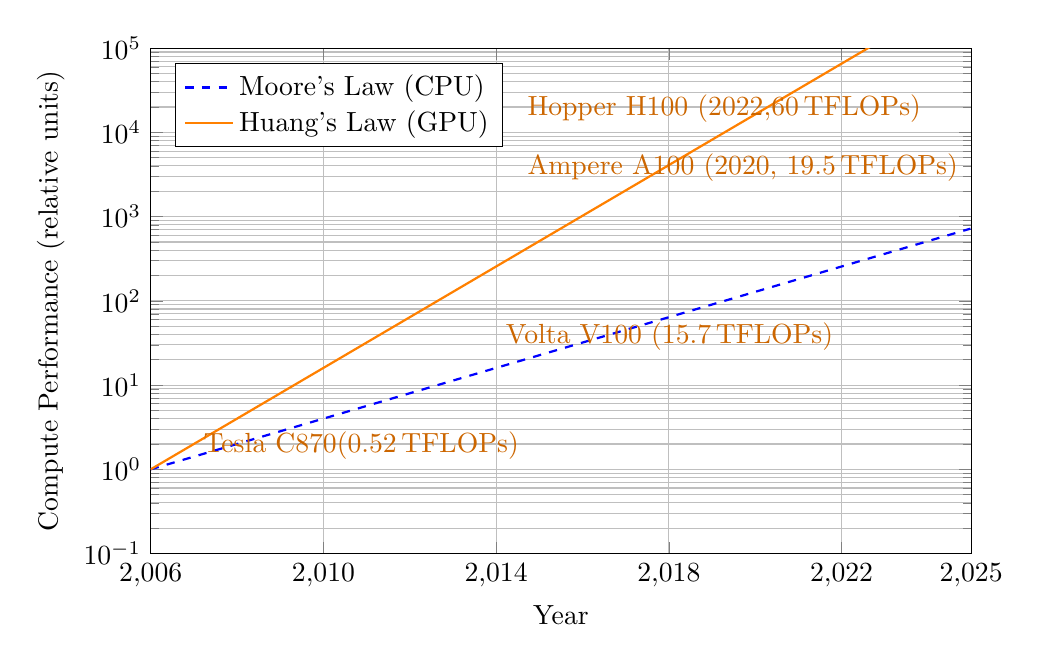
\begin{tikzpicture}
  \begin{semilogyaxis}[
    width=12cm, height=8cm,
    xlabel={Year},
    ylabel={Compute Performance (relative units)},
    xmin=2006, xmax=2025,
    ymin=0.1, ymax=1e5,
    xtick={2006,2010,2014,2018,2022,2025},
    grid=both,
    legend pos=north west,
    legend cell align=left,
    every axis plot/.append style={thick}
  ]

  % Moore's Law (doubling every two years)
  \addplot[
    blue, dashed, domain=2006:2025, samples=200
  ] {2^((x-2006)/2)};
  \addlegendentry{Moore's Law (CPU)}

  % Huang's Law (doubling every year)
  \addplot[
    orange, domain=2006:2025, samples=200
  ] {2^(x-2006)};
  \addlegendentry{Huang's Law (GPU)}

  % GPU Milestones
  \node[anchor=south west,orange!80!black] at (axis cs:2007,1) {Tesla C870(\SI{0.52}{TFLOPs})};
  \node[anchor=south west,orange!80!black] at (axis cs:2014,20) {Volta V100 (\SI{15.7}{TFLOPs})};
  \node[anchor=south west,orange!80!black] at (axis cs:2014.5,2000) {Ampere A100 (2020, \SI{19.5}{TFLOPs})};
  \node[anchor=south west,orange!80!black] at (axis cs:2014.5,10000) {Hopper H100 (2022,\SI{60}{TFLOPs})};
  \end{semilogyaxis}
\end{tikzpicture}

\end{frame}



\begin{frame}[plain,fragile]
\frametitle{Machine learning and AI models are computationally expensive}


% inline figure
\centerline{\includegraphics[width=1.0\linewidth]{figures/aitalk2.png}}

\end{frame}


\begin{frame}[plain,fragile]
\frametitle{And power greedy, perhaps quantum computers can reduce the impact?}

% inline figure
\centerline{\includegraphics[width=0.7\linewidth]{figures/aitalk1.png}}
Taken from \url{https://www.businessenergyuk.com/knowledge-hub/chatgpt-energy-consumption-visualized/}
\end{frame}

\begin{frame}
\frametitle{And perhaps not environmentally friendly}
\begin{itemize}
\item In Ireland, data centers consume more than 20 percent of the country’s electricity.
\item In Chile, precious aquifers are in danger of depletion.
\item In South Africa, where blackouts have long been routine, data centers are further taxing the national grid.
\item Similar concerns have surfaced in Brazil, Britain, India, Malaysia, the Netherlands, Singapore and Spain and other countries.
\end{itemize}
\end{frame}

\begin{frame}[plain,fragile]
\frametitle{The future is here, sooner than we may think}


% inline figure
\centerline{\includegraphics[width=1.05\linewidth]{figures/figuregoogle1.png}}

\end{frame}


\begin{frame}[plain,fragile]
\frametitle{Modern quantum platforms require cooling down to extremely low temperatures}


% inline figure
\centerline{\includegraphics[width=1.05\linewidth]{figures/miningthemoon.png}}

\end{frame}


\section{Introduction to Machine Learning}
\begin{frame}{What is Machine Learning?}
Machine Learning (ML) is the study of algorithms that improve through data experience.

\textbf{Types of Machine Learning:}
\begin{itemize}
    \item \textbf{Supervised Learning:} Labeled data for classification or regression.
    \item \textbf{Unsupervised Learning:} No labels; discover hidden patterns.
    \item \textbf{Reinforcement Learning:} Learning through interaction with the environment.
\end{itemize}


\textbf{ML Workflow:}
\[
\text{Data} \rightarrow \text{Model Training} \rightarrow \text{Prediction}
\]
\end{frame}




\begin{frame}[plain,fragile]
\frametitle{AI/ML and some statements you may have heard (and what do they mean?)}



\begin{enumerate}
\item Fei-Fei Li on ImageNet: \textbf{map out the entire world of objects} (\href{{https://cacm.acm.org/news/219702-the-data-that-transformed-ai-research-and-possibly-the-world/fulltext}}{The data that transformed AI research})

\item Russell and Norvig in their popular textbook: \textbf{relevant to any intellectual task; it is truly a universal field} (\href{{http://aima.cs.berkeley.edu/}}{Artificial Intelligence, A modern approach})

\item Woody Bledsoe puts it more bluntly: \textbf{in the long run, AI is the only science} (quoted in Pamilla McCorduck, \href{{https://www.pamelamccorduck.com/machines-who-think}}{Machines who think})
\end{enumerate}

\noindent
If you wish to have a critical read on AI/ML from a societal point of view, see \href{{https://www.katecrawford.net/}}{Kate Crawford's recent text Atlas of AI}.

\textbf{Here: with AI/ML we intend a collection of machine learning methods with an emphasis on statistical learning and data analysis}
\end{frame}







\begin{frame}[plain,fragile]
\frametitle{Main categories of Machine Learning}

\begin{block}{}
Another way to categorize machine learning tasks is to consider the desired output of a system.
Some of the most common tasks are:

\begin{itemize}
  \item Classification: Outputs are divided into two or more classes. The goal is to   produce a model that assigns inputs into one of these classes. An example is to identify  digits based on pictures of hand-written ones. Classification is typically supervised learning.

  \item Regression: Finding a functional relationship between an input data set and a reference data set.   The goal is to construct a function that maps input data to continuous output values.

  \item Clustering: Data are divided into groups with certain common traits, without knowing the different groups beforehand.  It is thus a form of unsupervised learning.
\end{itemize}

\noindent
\end{block}
\end{frame}





\begin{frame}[plain,fragile]
\frametitle{The plethora  of machine learning algorithms/methods}

\begin{enumerate}
\item Deep learning: Neural Networks (NN), Convolutional NN, Recurrent NN, Boltzmann machines, autoencoders and variational autoencoders  and generative adversarial networks, stable diffusion and many more generative models

\item Bayesian statistics and Bayesian Machine Learning, Bayesian experimental design, Bayesian Regression models, Bayesian neural networks, Gaussian processes and much more

\item Dimensionality reduction (Principal component analysis), Clustering Methods and more

\item Ensemble Methods, Random forests, bagging and voting methods, gradient boosting approaches 

\item Linear and logistic regression, Kernel methods, support vector machines and more

\item Reinforcement Learning; Transfer Learning and more 
\end{enumerate}

\noindent
\end{frame}





\begin{frame}[plain,fragile]
\frametitle{Example of discriminative modeling, \href{{https://www.oreilly.com/library/view/generative-deep-learning/9781098134174/ch01.html}}{taken from Generative Deep Learning by David Foster}}

\vspace{6mm}

% inline figure
\centerline{\includegraphics[width=1.0\linewidth]{figures/standarddeeplearning.png}}

\vspace{6mm}
\end{frame}

\begin{frame}[plain,fragile]
\frametitle{Example of generative modeling, \href{{https://www.oreilly.com/library/view/generative-deep-learning/9781098134174/ch01.html}}{taken from Generative Deep Learning by David Foster}}

\vspace{6mm}

% inline figure
\centerline{\includegraphics[width=1.0\linewidth]{figures/generativelearning.png}}

\vspace{6mm}
\end{frame}

\begin{frame}[plain,fragile]
\frametitle{Taxonomy of generative deep learning, \href{{https://www.oreilly.com/library/view/generative-deep-learning/9781098134174/ch01.html}}{taken from Generative Deep Learning by David Foster}}

\vspace{6mm}

% inline figure
\centerline{\includegraphics[width=1.0\linewidth]{figures/generativemodels.png}}

\vspace{6mm}
\end{frame}


\begin{frame}[plain,fragile]
\frametitle{What are the basic Machine Learning ingredients?}

\begin{block}{}
Almost every problem in ML and data science starts with the same ingredients:
\begin{itemize}
\item The dataset $\bm{x}$ (could be some observable quantity of the system we are studying)

\item A model which is a function of a set of parameters $\bm{\alpha}$ that relates to the dataset, say a likelihood  function $p(\bm{x}\vert \bm{\alpha})$ or just a simple model $f(\bm{\alpha})$

\item A so-called \textbf{loss/cost/risk} function $\mathcal{C} (\bm{x}, f(\bm{\alpha}))$ which allows us to decide how well our model represents the dataset. 
\end{itemize}

\noindent
We seek to minimize the function $\mathcal{C} (\bm{x}, f(\bm{\alpha}))$ by finding the parameter values which minimize $\mathcal{C}$. This leads to  various minimization algorithms. It may surprise many, but at the heart of all machine learning algortihms there is an optimization problem. 
\end{block}
\end{frame}


\begin{frame}[plain,fragile]
\frametitle{\href{{https://journals.aps.org/prresearch/pdf/10.1103/PhysRevResearch.5.033062}}{Dilute neutron star matter from neural-network quantum states by Fore {\em et al.}, Physical Review Research 5, 033062 (2023)} at density $\rho=0.04$ fm$^{-3}$}

\centerline{\includegraphics[width=0.9\linewidth]{figures/nmatter.png}}

\end{frame}









\begin{frame}{What is quantum technology? Three main fields}
\begin{block}{Quantum computing} is a new computing paradigm that capitalizes on the laws of quantum mechanics to provide significant performance improvement for certain applications, and to enable new territories of computing beyond existing classical
computing.
\end{block}
\begin{block}{Quantum communication} is the secure transfer of quantum information across distances and could ensure security ofcommunication even in the face of unlimited quantum computing power.
\end{block}    
\begin{block}{Quantum sensing} includes a new generation of sensors, based on quantum systems, that provide measurements of various
quantities (for example, electromagnetic fields, gravity, or time) and that are orders of magnitude more sensitive than classical
sensors.
\end{block}
\end{frame}


\begin{frame}[plain,fragile]
\frametitle{Where are we?}


% inline figure
\centerline{\includegraphics[width=1.05\linewidth]{figures/cartoonqc.png}}

\end{frame}





%-----------------------------------------------------------
%\section{Introduction to Quantum Computing}
\begin{frame}{The basic concepts}
Quantum technologies leverage principles of quantum mechanics to perform computations beyond classical capabilities.

\vspace{10pt}
\textbf{Key Concepts:}
\begin{itemize}
\item \textbf{Superposition:} Qubits can exist in a combination of states.
\item \textbf{Entanglement:} Correlation between qubits regardless of distance.
\item \textbf{Quantum Interference:} Probability amplitudes interfere. Is a core tool in quantum algorithms. It is used to amplify the probability of finding the correct answer while suppressing incorrect ones.
\end{itemize}

\end{frame}

\begin{frame}{Superposition}

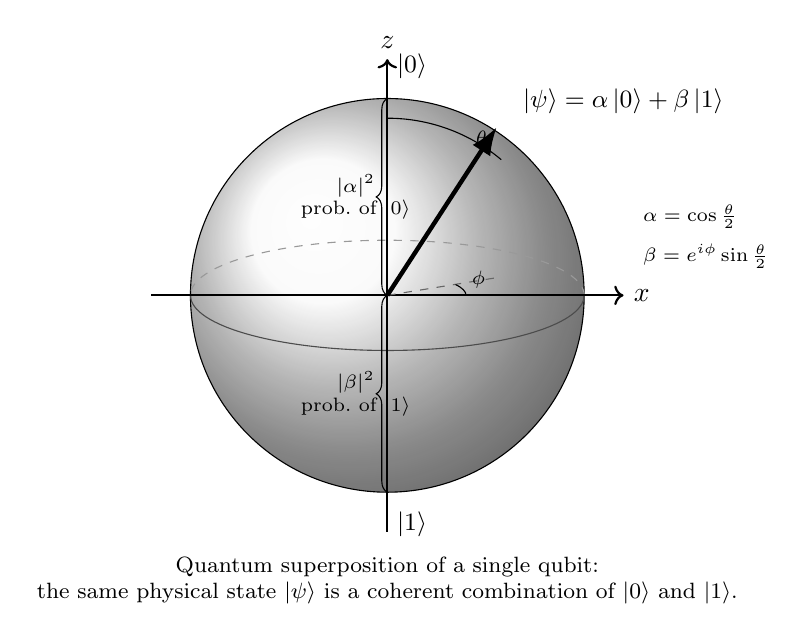
\begin{tikzpicture}[scale=2.5,
   axis/.style={->, thick},
   basislabel/.style={anchor=south east, inner sep=1pt, font=\small},
   statelabel/.style={anchor=west, font=\small},
   myvec/.style={-Latex, thick},
]

% Bloch sphere
\shade[ball color=white!95!gray, opacity=0.9] (0,0) circle (1cm);
\draw[thin, black] (0,0) circle (1cm);

% Draw "equator" ellipse (x-y plane)
\draw[thin, black!70] (-1,0) arc[start angle=180, end angle=360, x radius=1cm, y radius=0.28cm];
\draw[dashed, thin, black!40] (1,0) arc[start angle=0, end angle=180, x radius=1cm, y radius=0.28cm];

% Axes
\draw[axis] (0,-1.2) -- (0,1.2) node[above] {$z$};
\draw[axis] (-1.2,0) -- (1.2,0) node[right] {$x$};

% Poles: |0> at +z, |1> at -z
\node[font=\small, anchor=south west] at (0,1.05) {$\ket{0}$};
\node[font=\small, anchor=north west] at (0,-1.05) {$\ket{1}$};

% State vector |ψ>
% We'll pick some angles θ and φ.
% θ = polar angle from +z, φ = azimuth in x-y plane.
% Say θ = 40°, φ = 30°
\pgfmathsetmacro{\th}{40}   % polar
\pgfmathsetmacro{\ph}{30}   % azimuth
\pgfmathsetmacro{\xp}{sin(\th)*cos(\ph)}
\pgfmathsetmacro{\yp}{0.28*sin(\th)*sin(\ph)} % projected y (ellipse scaling)
\pgfmathsetmacro{\zp}{cos(\th)}

% draw projection of state onto equator
\draw[dashed, black!60] (0,0) -- (\xp,\yp);

% state vector
\draw[myvec, ultra thick] (0,0) -- (\xp,\yp+\zp);

% angle θ from +z axis
\draw[thin] (0,0.9) arc[start angle=90, end angle={90-\th}, radius=0.9cm];
\node[font=\scriptsize, anchor=west] at (0.4,0.8) {$\theta$};

% angle φ in x-y plane
\draw[thin] (0.4,0) arc[start angle=0, end angle=\ph, x radius=0.4cm, y radius=0.11cm];
\node[font=\scriptsize, anchor=west] at (0.38,0.08) {$\phi$};

% Label the state vector
\node[statelabel] at ($(0,0)!1.15!(\xp,\yp+\zp)$) {$\ket{\psi} =
\alpha\ket{0} + \beta\ket{1}$};

% Show alpha,beta magnitudes as cos(θ/2), sin(θ/2)
\node[font=\scriptsize, align=left, anchor=west] at (1.25,0.4) {$\alpha = \cos\frac{\theta}{2}$};
\node[font=\scriptsize, align=left, anchor=west] at (1.25,0.2) {$\beta = e^{i\phi}\sin\frac{\theta}{2}$};

% Little braces showing probabilities
\draw[decorate,decoration={brace, amplitude=4pt}]
 (0,0) -- (0,1)
 node[midway, xshift=-0.4cm, font=\scriptsize, align=center]
 {$|\alpha|^2$\\prob.\ of $\ket{0}$};

\draw[decorate,decoration={brace, amplitude=4pt}]
 (0,-1) -- (0,0)
 node[midway, xshift=-0.4cm, font=\scriptsize, align=center]
 {$|\beta|^2$\\prob.\ of $\ket{1}$};

% Caption under figure
\node[font=\footnotesize, align=center] at (0,-1.45)
{Quantum superposition of a single qubit:\\
the same physical state $\ket{\psi}$ is a coherent combination
of $\ket{0}$ and $\ket{1}$.};

\end{tikzpicture}
\end{frame}


\begin{frame}{What is Quantum Entanglement?}
\textbf{Quantum Entanglement} is a quantum phenomenon where two or more particles become correlated in such a way that the state of one particle directly affects the state of the other, regardless of distance. Fundamental for making quantum gates, quantum sensors and much more. 

\vspace{10pt}
\textbf{Key Features:}
\begin{itemize}
    \item Non-local correlations
    \item No classical analog
\end{itemize}

\end{frame}


\begin{frame}{Entanglement}
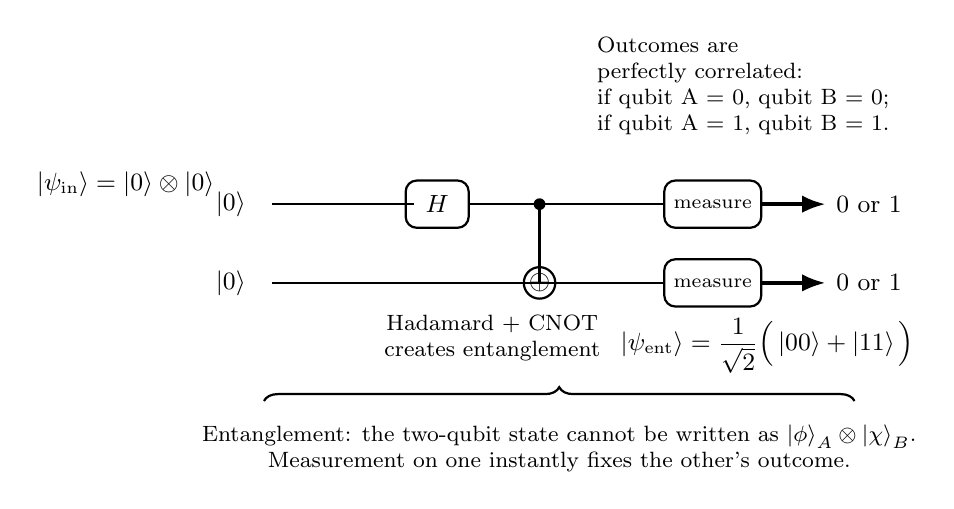
\begin{tikzpicture}[
   thick,
   wire/.style={thick},
   gate/.style={draw, rounded corners, minimum width=0.8cm, minimum height=0.6cm, font=\small, fill=white},
   ctrl/.style={fill=black, circle, inner sep=1.5pt},
   target/.style={draw, circle, inner sep=0pt, minimum width=0.4cm},
   measure/.style={draw, rounded corners, minimum width=0.9cm, minimum height=0.6cm, font=\scriptsize, fill=white},
   amp/.style={-Latex, very thick},
   note/.style={font=\small},
   outcome/.style={font=\small, align=center},
   corr/.style={font=\footnotesize},
]

%%%% 1. LEFT: Initial product state %%%%

\node[note, anchor=east] (psi0label) at (-0.4,0.75)
{$\displaystyle \ket{\psi_\text{in}} = \ket{0}\otimes\ket{0}$};

% Input kets (two wires)
\node[note, anchor=east] (q0in) at (0,0.5) {$\ket{0}$};
\node[note, anchor=east] (q1in) at (0,-0.5) {$\ket{0}$};

% Horizontal wires (input region to circuit region)
\draw[wire] (0.2,0.5) -- (2.0,0.5);
\draw[wire] (0.2,-0.5) -- (2.0,-0.5);

%%%% 2. CIRCUIT: H on top, then CNOT %%%%

% Hadamard gate on first qubit
\node[gate] (Hgate) at (2.3,0.5) {$H$};

\draw[wire] (2.0,0.5) -- (Hgate.west);
\draw[wire] (Hgate.east) -- (3.2,0.5);

% Vertical line for CNOT control-target
\draw[wire] (3.6,0.5) -- (3.6,-0.5);

% Control dot on top wire
\node[ctrl] (ctrl) at (3.6,0.5) {};

% Target ⊕ on bottom wire
\node[target] (targ) at (3.6,-0.5) {$\oplus$};

% extend wires to the right of CNOT
\draw[wire] (3.2,0.5) -- (4.2,0.5);
\draw[wire] (2.0,-0.5) -- (4.2,-0.5);

% Label under circuit: "Entangling operation"
\node[font=\footnotesize, align=center] at (3.0,-1.2)
{Hadamard + CNOT\\creates entanglement};

%%%% 3. STATE AFTER CIRCUIT %%%%

\node[note, anchor=west] (psiBell) at (4.5,-1.3)
{$\displaystyle
\ket{\psi_\text{ent}} =
\frac{1}{\sqrt{2}}\Big(\ket{00}+\ket{11}\Big)
$};

%%%% 4. MEASUREMENT BOXES %%%%

% Measurement boxes on each qubit
\node[measure] (M0) at (5.8,0.5) {measure};
\node[measure] (M1) at (5.8,-0.5) {measure};

% wires into measurement
\draw[wire] (4.2,0.5) -- (M0.west);
\draw[wire] (4.2,-0.5) -- (M1.west);

% classical arrows out
\draw[amp] (M0.east) -- ++(0.8,0.0) node[outcome, anchor=west]
{$0$ or $1$};
\draw[amp] (M1.east) -- ++(0.8,0.0) node[outcome, anchor=west]
{$0$ or $1$};

% Correlation annotation
\node[corr, align=left, anchor=west] at (4.2,2.0)
{Outcomes are\\perfectly correlated:\\
if qubit A = 0, qubit B = 0;\\
if qubit A = 1, qubit B = 1.};

%%%% 5. BIG BRACE + TEXT EXPLANATION %%%%

% Decorative brace under entire figure
\draw[decorate, decoration={brace, amplitude=5pt}]
 (0.1,-2.0) -- (7.6,-2.0)
 node[midway, yshift=-0.6cm, align=center, font=\footnotesize]
 {Entanglement: the two-qubit state cannot be written
  as $\ket{\phi}_A \otimes \ket{\chi}_B$.\\
  Measurement on one instantly fixes the other's outcome.};

\end{tikzpicture}
\end{frame}

}


\begin{frame}{Interference}

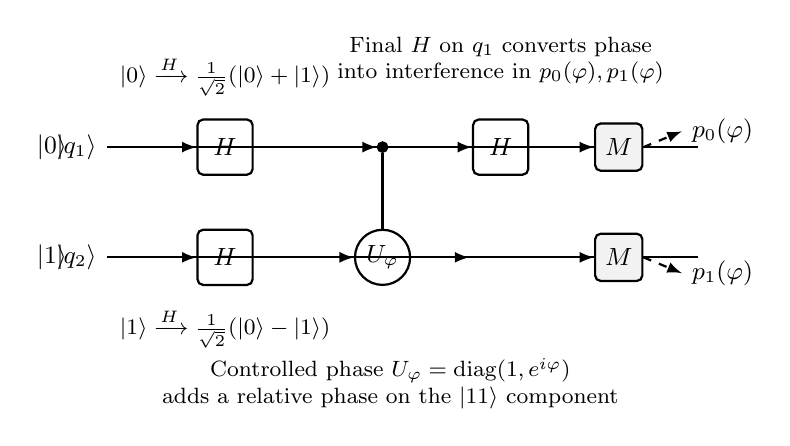
\begin{tikzpicture}[
    >=latex,
    thick,
    gate/.style={draw, rectangle, minimum width=7mm, minimum height=7mm, rounded corners=2pt},
    phasegate/.style={draw, circle, minimum size=7mm, inner sep=0pt},
    meas/.style={draw, rectangle, minimum width=6mm, minimum height=6mm, rounded corners=2pt, fill=gray!10},
    control/.style={draw, fill=black, circle, inner sep=1.2pt},
    line/.style={},
    every node/.style={font=\small}
]

% Horizontal positions
\def\xinit{0.0}
\def\xHone{1.5}
\def\xphase{3.5}
\def\xHtwo{5.0}
\def\xmeas{6.5}

% Vertical positions
\def\yqone{0.7}
\def\yqtwo{-0.7}

% Qubit labels
\node[left] at (\xinit,\yqone) {$\lvert q_1 \rangle$};
\node[left] at (\xinit,\yqtwo) {$\lvert q_2 \rangle$};

% Initial states (|0> and |1>)
\node at (\xinit-0.7,\yqone) {$\lvert 0 \rangle$};
\node at (\xinit-0.7,\yqtwo) {$\lvert 1 \rangle$};

% Wires
\draw (\xinit,\yqone) -- (\xmeas+1.0,\yqone);
\draw (\xinit,\yqtwo) -- (\xmeas+1.0,\yqtwo);

% First layer: Hadamard on both qubits
\node[gate] (H1) at (\xHone,\yqone) {$H$};
\node[gate] (H2) at (\xHone,\yqtwo) {$H$};

\draw[->] (\xinit+0.1,\yqone) -- (H1.west);
\draw[->] (\xinit+0.1,\yqtwo) -- (H2.west);

% Controlled phase U_phi on second qubit, controlled by first
\node[control] (C) at (\xphase,\yqone) {};
\node[phasegate] (P) at (\xphase,\yqtwo) {$U_\varphi$};

\draw (C) -- (P);
% input from H gates to control and target
\draw[->] (H1.east) -- (C.west);
\draw[->] (H2.east) -- (P.west);

% Second Hadamard on control qubit (to reveal interference)
\node[gate] (H3) at (\xHtwo,\yqone) {$H$};
\draw[->] (C.east) -- (H3.west);
\draw[->] (P.east) -- (\xHtwo-0.4,\yqtwo);

% Measurements
\node[meas] (M1) at (\xmeas,\yqone) {$M$};
\node[meas] (M2) at (\xmeas,\yqtwo) {$M$};

\draw[->] (H3.east) -- (M1.west);
\draw[->] (\xHtwo+0.2,\yqtwo) -- (M2.west);

% Classical readout arrows (just decorative)
\draw[->, dashed] (M1.east) -- (\xmeas+0.8,\yqone+0.2) node[right] {$p_0(\varphi)$};
\draw[->, dashed] (M2.east) -- (\xmeas+0.8,\yqtwo-0.2) node[right] {$p_1(\varphi)$};

% Annotations: superposition & phase kickback
\node[align=left, font=\footnotesize] at (1.5,1.6)
    {$\lvert 0\rangle \xrightarrow{H} \tfrac{1}{\sqrt{2}}(\lvert 0\rangle + \lvert 1\rangle)$};
\node[align=left, font=\footnotesize] at (1.5,-1.6)
    {$\lvert 1\rangle \xrightarrow{H} \tfrac{1}{\sqrt{2}}(\lvert 0\rangle - \lvert 1\rangle)$};

\node[align=center, font=\footnotesize] at (3.6,-2.3)
    {Controlled phase $U_\varphi = \mathrm{diag}(1, e^{i\varphi})$\\
     adds a relative phase on the $\lvert 11\rangle$ component};

\node[align=center, font=\footnotesize] at (5.0,1.8)
    {Final $H$ on $q_1$ converts phase\\
     into interference in $p_0(\varphi), p_1(\varphi)$};

\end{tikzpicture}


\end{frame}





\begin{frame}{Quantum Speedups}
\textbf{Why Quantum?}
\begin{itemize}
    \item \textbf{Quantum Parallelism:} Process multiple states simultaneously.
    \item \textbf{Quantum Entanglement:} Correlated states for richer information.
    \item \textbf{Quantum Interference:} Constructive and destructive interference to enhance solutions, is a core tool in quantum algorithms. 
\end{itemize}

\textbf{Example - Grover's Algorithm:}
\[
\text{Quantum Search Complexity: } O(\sqrt{N}) \text{ vs. } O(N)
\]

\textbf{Advantage:}
- Speedups in high-dimensional optimization and linear algebra problems.
\end{frame}


%-----------------------------------------------------------
%\section{Challenges in Quantum Machine Learning}
\begin{frame}{Challenges and Limitations}
\textbf{1. Quantum Hardware Limitations:}
\begin{itemize}
    \item Noisy Intermediate-Scale Quantum (NISQ) devices.
    \item Decoherence and limited qubit coherence times.
\end{itemize}

\textbf{2. Data Encoding:}
\begin{itemize}
    \item Efficient embedding of classical data into quantum states.
\end{itemize}

\textbf{3. Scalability:}
\begin{itemize}
    \item Difficult to scale circuits to large datasets.
\end{itemize}
\end{frame}






\begin{frame}{1. Quantum Communication}
\textbf{Quantum Teleportation:}
\begin{itemize}
    \item Entanglement enables the transmission of quantum states using classical communication.
    \item No need to send the physical quantum particle.
\end{itemize}

\textbf{Advantage:}
\begin{itemize}
\item Instantaneous state transfer within quantum mechanics constraints.
\item Quantum networks rely on entanglement for secure communication.
  \end{itemize}
\end{frame}

\begin{frame}{2. Quantum Cryptography}
\textbf{Quantum Key Distribution:}
\begin{itemize}
    \item Entanglement ensures secure communication.
    \item Eavesdropping disturbs quantum states, revealing interception attempts.
\end{itemize}

\begin{itemize}
\item Any measurement by a third party collapses the wavefunction.  
\item Ensures security based on quantum mechanics, not computational hardness.
\end{itemize}
\textbf{Advantage:} Unconditional security guaranteed by the laws of physics.
\end{frame}

\begin{frame}{3. Quantum Computing}
\textbf{Speedup in Quantum Algorithms:}
\begin{itemize}
    \item Entanglement provides exponential state space.
    \item Quantum parallelism arises from entangled qubits.
\end{itemize}

\textbf{Grover's Algorithm:}
\[
\mathcal{O}(\sqrt{N}) \text{ vs. } \mathcal{O}(N)
\]

\textbf{Shor's Algorithm:}
\[
\text{Factoring in } \mathcal{O}((\log N)^3)
\]
\end{frame}

\begin{frame}[plain,fragile]
\frametitle{4. Quantum Metrology}

\textbf{Quantum Metrology:}
\begin{itemize}
    \item Uses entangled states for ultra-precise measurements.
    \item Overcomes the classical shot-noise limit.
\end{itemize}

\textbf{Heisenberg Limit:}
\[
\Delta \theta \ge \frac{1}{N},
\]

where \( N \) is the number of entangled particles.  

\begin{block}{Advantage:}
\begin{itemize}
\item Quantum entanglement improves sensitivity beyond classical limits.
\end{itemize}
\end{block}
\end{frame}

\begin{frame}{Challenges of Quantum Entanglement}
\textbf{Decoherence:}
\begin{itemize}
    \item Entangled states are fragile.
    \item Interaction with the environment collapses the wavefunction.
\end{itemize}

\textbf{Scalability:}
\begin{itemize}
    \item Difficult to entangle large numbers of qubits.
    \item Error correction requires complex protocols.
\end{itemize}

\textbf{Measurement Problem:}
\begin{itemize}
    \item Measurement destroys entanglement.
    \item Trade-off between information gain and entanglement preservation.
\end{itemize}
\end{frame}

%-----------------------------------------------------------
%\section{Quantum Machine Learning (QML)}
\begin{frame}{What is Quantum Machine Learning?}
\textbf{Quantum Machine Learning (QML)} integrates quantum computing with machine learning algorithms to exploit quantum advantages.

\vspace{10pt}
\textbf{Motivation:}
\begin{itemize}
    \item High-dimensional Hilbert spaces for better feature representation.
    \item Quantum parallelism for faster computation.
    \item Quantum entanglement for richer data encoding.
\end{itemize}


\end{frame}



\begin{frame}[plain,fragile]
\frametitle{Di Vincenzo criteria}

\begin{alertblock}{Quantum computing requirements}
\begin{enumerate}
\item A scalable physical system with well-characterized qubit

\item The ability to initialize the state of the qubits to a simple fiducial state

\item Long relevant Quantum coherence times longer than the gate operation time

\item A \textbf{universal} set of quantum gates

\item A qubit-specific measurement capability
\end{enumerate}

\noindent
\end{alertblock}
\end{frame}

\begin{frame}[plain,fragile]
\frametitle{Quantum platforms}

\begin{enumerate}
\item Superconducting qubits use Josephson junction circuits operated at millikelvin temperatures
\item Trapped-ion computers confine ions (e.g.\ $^{171}$Yb$^+$, $^{40}$Ca$^+$) in electromagnetic traps, encoding qubits in internal electronic states. Gates are implemented with laser or microwave fields coupling to vibrational modes.
\item Photonic quantum computing employs photons (in dual-rail or  continuous-variable encodings) as qubits
\item Spin qubits—realized in silicon quantum dots, donor atoms, or color centers—encode information in electron or nuclear spin states.
  \item Electrons on helium/neon (more on this below, own research)

\end{enumerate}


\end{frame}


\begin{frame}[plain,fragile]
\frametitle{Where are we? More seriously}


% inline figure
\centerline{\includegraphics[width=1.05\linewidth]{figures/wherearewe.png}}

\end{frame}


\begin{frame}[plain,fragile]
\frametitle{Where are we? More seriously}


% inline figure
\centerline{\includegraphics[width=1.05\linewidth]{figures/presentday.png}}

\end{frame}


\section{The next decade}

\begin{frame}[plain,fragile]
\frametitle{Considerable investements (McKinsey Quantum Technology Monitor, June 2025 )}


% inline figure
\centerline{\includegraphics[width=0.9\linewidth]{qcfigures/image1.png}}

\end{frame}


\begin{frame}[plain,fragile]
\frametitle{Quantum technology (QT) investments by funding type, 2014–24}


% inline figure
\centerline{\includegraphics[width=0.9\linewidth]{qcfigures/image2.png}}

\end{frame}

\begin{frame}[plain,fragile]
\frametitle{Announcements of public investments in quantum technology }


% inline figure
\centerline{\includegraphics[width=0.9\linewidth]{qcfigures/image3.png}}

\end{frame}

\begin{frame}[plain,fragile]
\frametitle{The United States and Japan lead other countries in the number of patents
granted for quantum technology}


% inline figure
\centerline{\includegraphics[width=1.0\linewidth]{qcfigures/image4.png}}

\end{frame}

\begin{frame}[plain,fragile]
\frametitle{The United States and China lead other countries in the number of filed patents}


% inline figure
\centerline{\includegraphics[width=1.0\linewidth]{qcfigures/image5.png}}

\end{frame}


\begin{frame}[plain,fragile]
\frametitle{The quantum communication market is projected to reach 11 billion to
15 billion USD by 2035.}


% inline figure
\centerline{\includegraphics[width=0.9\linewidth]{qcfigures/image6.png}}

\end{frame}



    

\section{Legal aspects and export control resrictions}



\frame
    {
      \frametitle{New platform: electrons on helium, \url{https://eeroq.com/}}

      \begin{footnotesize}
     \begin{columns}
       \column{5.0cm}
\begin{enumerate}
\item Long coherence times

\item Highly connected qubits

\item Many and controllable qubits in a small area

\item CMOS compatible

\item Fast gates
\end{enumerate}

\column{6cm}
      \begin{center}
        \rotatebox[origin=c]{-90}{\includegraphics[width=1.3\textwidth]{qcfigures/lab.jpeg}}
      \end{center}
\end{columns}
      \end{footnotesize}
    }





\frame
    {
      \frametitle{Single electrons can make great qubits}
	
      \begin{footnotesize}
     \begin{columns}
       \column{5.0cm}

       At the heart is the trapping and control
       of individual electrons floating above pools of superfluid
       helium. These electrons form the qubits of our quantum
       computer, and the purity of the superfluid helium protects the
       intrinsic quantum properties of each electron. The  ultimate
       goal is to build a large-scale quantum computer based on
       quantum magnetic (spin) state of these trapped electrons.
\column{5cm}
      \begin{center}
	\includegraphics[width=1.2\textwidth]{qcfigures/nordicquantumfig1.png}
      \end{center}
\end{columns}
      \end{footnotesize}
    }


\frame
    {
      \frametitle{Trapping electrons in microchannels}
	
      \begin{footnotesize}
     \begin{columns}
       \column{5.0cm}
Microchannels fabricated into silicon wafers are filled with superfluid helium and energized electrodes. Together with the natural electron trapping properties of superfluid helium, these allow for the precision trapping of individual or multiple electrons. The microchannels are only a few micrometers in size, or about five times smaller than the diameter of a human hair.
\column{5cm}
      \begin{center}
	\includegraphics[width=1.2\textwidth]{qcfigures/nordicquantumfig2.png}
      \end{center}
\end{columns}
      \end{footnotesize}
    }

\frame
    {
      \frametitle{Control and readout}
	
      \begin{footnotesize}
     \begin{columns}
       \column{5.0cm}

       Microchannel regions can store thousands of electrons, from which one can be plucked and transported to the single electron control and readout area. In this region, microwave signals will interact with the electron to perform quantum logic gate operations, which will be readout via extremely fast electronics.


\column{5cm}
      \begin{center}
	\includegraphics[width=1.2\textwidth]{qcfigures/nordicquantumfig3.png}
      \end{center}
\end{columns}
      \end{footnotesize}
    }


\frame
    {
      \frametitle{Operations for quantum computing}
	
      \begin{footnotesize}
     \begin{columns}
       \column{5.0cm}
Quantum information can be encoded in a number of ways using single electrons. Currently, we are working with the side-to-side(lateral) quantum motion of the electron in the engineered trap. This motion can either be in its lowest energy state, the ground state, or in a number of higher-energy excited states. This electron motion also provides the readout capabilities for the ultimate goal of building a large-scale quantum computer based on the electron's magnetic moment (spin).       
\column{5cm}
      \begin{center}
	\includegraphics[width=1.2\textwidth]{qcfigures/nordicquantumfig4.png}
      \end{center}
\end{columns}
      \end{footnotesize}
    }
    
\begin{frame}[plain,fragile]
\frametitle{New export control rules}
\begin{block}{}
The US Bureau of Industry and Security (BIS) rules are new export
controls on certain quantum computing items, implemented through an
Interim Final Rule (IFR) on September 6, 2024. These rules add
worldwide licensing requirements for items on the Commerce Control
List (CCL), create a new license exception for allied countries, and
establish reporting requirements. The aim is to control the export of
advanced technologies, including quantum computing components,
software, and equipment, for national security and foreign policy
reasons.
\end{block}

\end{frame}


\begin{frame}[plain,fragile]
\frametitle{What is controlled}
\begin{block}{}
\begin{itemize}
\item Quantum computing items: This includes computers, software, components, materials, and related equipment used in their development and maintenance.
\item Advanced semiconductor manufacturing equipment: Tools and machines for producing advanced chips.
\item Technology: Technology for high-performance computing chips.
Additive manufacturing items: Equipment for producing metal components.
\end{itemize}
\end{block}

\end{frame}




\begin{frame}[plain,fragile]
\frametitle{Export control, selected list from own collaborations}
\begin{block}{Technology/Component and Reason for Sensitivity}
\begin{itemize}
\item Superconducting CPW resonator: Advanced quantum sensor with potential defense/communications applications.
\item Single-electron trap (gated microchannel): Specialized microelectronic architecture for quantum computing. 
\item Superconducting electrodes (Nb films):  Superconducting materials in high-Q resonators and quantum circuits. 
\item Superfluid $^4$He substrate:  Specialized cryogenic environment and novel quantum materials. 
\item Cryogenic RF components:  Similar hardware is used in radar and communications systems.
\item Electron-on-helium qubit platform: Emerging quantum information platform targeted by new export controls; potential secure/advanced computation application. 
\end{itemize}
\end{block}
\end{frame}

\begin{frame}[plain,fragile]
\frametitle{Other topics to discuss}
\begin{itemize}
\item Quantum Technologies and International Treaties
\item Quantum computing raises questions about whether existing statutes on intellectual property, liability, privacy, and even antitrust are adequate 
\item Cybersecurity in the Quantum Era: Threats and Legal Responses – How quantum computing jeopardizes current cryptography and what laws can do about it
\item Quantum Communication and Privacy
\item Quantum Sensing and Surveillance: Privacy and  National Security Implications
\item Export Controls and Quantum Tech: Balancing Security and Innovation
\item Patents and IP in the Quantum Era: Innovation vs. Open Science
\item Geopolitics of Quantum: The New Tech Arms Race and Legal Strategy
\item Ethical Quantum Technologies: Ensuring Responsible Innovation and many more
\end{itemize}

\end{frame}

\begin{frame}[plain,fragile]
\frametitle{Observations (or conclusions if you prefer)}


\begin{block}{}
\begin{itemize}
\item How do we develop insights, competences, knowledge in AI and quantum technologies  that can advance a given field?
\begin{itemize}

  \item For example: Can we use ML to find out which correlations are relevant and thereby diminish the dimensionality problem in complex interacting  many-particle systems?

  \item Can we use AI/ML in detector analysis, accelerator design, analysis of experimental data and more?

  \item Can we use AL/ML to carry out reliable extrapolations by using current experimental knowledge and current theoretical models?
\item How do we study entanglement in various quantum platforms? Can we use AI/ML for better design?

\end{itemize}

\noindent
\item The community needs to invest in relevant educational efforts and training of scientists with knowledge in AI/ML and quantum technologies

\item Most likely tons of things I have forgotten
\end{itemize}

\noindent
\end{block}
\end{frame}

\begin{frame}{Selected applications of Quantum Machine Learning}
\textbf{1. Quantum mechanical many-particle systems:}
\begin{itemize}
    \item Simulate  structures in nuclei, atoms, moleculs etc with QML.
\end{itemize}

\textbf{2. Finance:}
\begin{itemize}
    \item Quantum optimization for portfolio management.
\end{itemize}

\textbf{3. Image Recognition:}
\begin{itemize}
    \item Quantum-enhanced convolutional neural networks.
\end{itemize}
\end{frame}



\begin{frame}{Future Perspectives}
\textbf{Quantum Internet:}
\begin{itemize}
    \item Entanglement as a resource for global quantum networks.
\end{itemize}

\textbf{Fault-Tolerant Quantum Computing:}
\begin{itemize}
    \item Quantum error correction leveraging entanglement.
\end{itemize}

\textbf{Advanced Quantum Sensors:}
\begin{itemize}
    \item Improved sensitivity for medical and scientific applications.
\end{itemize}

\end{frame}
\end{document}













